\section{Polyline Simplification and Basic Properties}\label{sec:polyline-simplification}
In this section, we discuss and illustrate different types of simplification objectives that have been studied. This yields valuable insights for the rest of this work. It also highlights the differences between the previously studied types and the global (vertex-restricted) simplification under the Fréchet distance, which is our main focus.

We mainly use the classification of \citeauthor{global_curve_simplification}~\cite{global_curve_simplification} as a basis.

There are two key aspects in which simplification variants differ from each other:
\begin{enumerate}
  \item The set from which the points of the simplification are chosen.
	\item The distance function between polylines used to measure the quality of the simplification.
\end{enumerate}
These two aspects are not completely independent.

In \cref{sec:preliminaries}, we defined the \emph{Fréchet distance}. The other commonly used function is the \emph{Hausdorff distance}.

\begin{definition}[Hausdorff Distance]
  Let \(P\) and \(Q\) be polylines of length \(p\) and \(q\), respectively, in \(d\)-dimensional space. Let \(\delta\) be a distance function on points.
	\begin{itemize}
		\item The \emph{directed Hausdorff distance} \(\delta^{dH}(P, Q)\) from \(P\) to \(Q\) is defined as
		\[\delta^{dH}(P, Q) = \max_{s \in [0, p]}\min_{t \in [0, q]} \delta(P(s), Q(t)).\]
		\item The \emph{(undirected) Hausdorff distance} \(\delta^{H}(P, Q)\) between \(P\) and \(Q\) is defined as
		\[\delta^{H}(P, Q) = \max(\delta^{dH}(P, Q), \delta^{dH}(Q, P)).\]
	\end{itemize}
	Note that the directed Hausdorff distance is not symmetric, while the undirected Hausdorff distance is.
\end{definition}

The Hausdorff and Fréchet distances can be based on different point distances, with the most common being the Euclidean, Manhattan, and Chebyshev distances.

These distances measure the similarity between the simplification and the original polyline. In the case of the directed Hausdorff distance, it can be applied in two directions: from the simplification to the polyline or vice versa.

A common alternative for both the Hausdorff and Fréchet distances is to compare the simplification only \emph{locally}.

To understand local simplification, we need to define the allowed points for the simplification. Van de Kerkhof et al. distinguish three types of point selection:
\begin{itemize}
  \item \emph{Vertex-restricted}: Only the original vertices of the polyline are allowed. For a polyline \(P = \angl{u_0, \dots, u_n}\), a simplification must be a subsequence of \(u_0, \dots, u_n\) preserving the order.
	\item \emph{Curve-restricted}: Any point lying on the polyline is allowed. For a polyline \(P\) of length \(p\), any point \(P(t)\) for \(t \in [0, p]\) is valid. The sequence of parameters \(t\) must be increasing.
	\item \emph{Non-restricted}: Any point in the ambient space is valid.
\end{itemize}

Local simplification is mainly used in the vertex-restricted setting but also applies to the curve-restricted one. In this approach, the distance function is not applied globally between \(Q\) and \(P\). Instead, it is applied between each line segment of \(Q\) and its corresponding subpolyline in \(P\), and the maximum of these distances is taken. More specifically, for a polyline distance function \(\delta^P\), we define the local distance \(\delta^{LP}\) as
\[\delta^{LP}(P, Q) = \max_{i = 1, \dots, q} \delta^P(P[k_{i-1}\dots k_i], Q[i-1 \dots i]),\]
where \(P = \angl{u_0, \dots, u_p}\) and \(Q = \angl{u_{k_0}, \dots, u_{k_q}}\).

In contrast to the local setting, we study the \emph{global} Fréchet distance in this work. In the global setting, the non-restricted cases can also be considered.

In the following, we discuss the vertex-restricted local and global (undirected) Hausdorff and Fréchet variants. For more information on other global variants, we refer to \citeauthor{global_curve_simplification}'s paper.

\subsection{Hausdorff Distance}
In this thesis, we study only the Fréchet distance. The global Hausdorff distance is the least useful among the four variants discussed here. Van Kreveld et al. showed that finding such simplifications is NP-hard~\cite{on_optimal_polyline_simplification_using_the_hausdorff_and_frechet_distance}, making it impractical for applications. Furthermore, it does not capture the contour of a polyline well, as the order of points is not considered. This can lead to oversimplifications. See \cref{fig:polyline-ex-hausdorff} for an example illustrating why the Hausdorff distance may be problematic for measuring similarity.

\begin{figure}[b]
  \centering
  \includegraphics{./tikz-fig/polyline-ex-hausdorff.pdf}
  \caption{Two polylines with a comparatively high Fréchet distance but small Hausdorff distance. Each point on either polyline is close to some point on the other, resulting in a small Hausdorff distance. However, the completely different contours cause a high Fréchet distance.}
  \label{fig:polyline-ex-hausdorff}
\end{figure}

The local Hausdorff variant does not suffer from the same problems, as applying the Hausdorff distance locally enforces a coarse global order on the simplification. Moreover, while the global Hausdorff variant is the hardest to solve, the local Hausdorff setting appears to be the simplest. Currently, it is the only variant for which subcubic algorithms are known in dimensions \(d \geq 3\) (see, e.g., \cite{efficiently_approximating_higher_dim}).

The local Hausdorff variant has already been covered extensively, so we do not expand further on it.

\subsection{Local Fréchet}
The local Fréchet variant enforces locality constraints similar to the local Hausdorff variant but uses the Fréchet distance. Unlike the Hausdorff distance, the Fréchet distance inherently enforces the correct point ordering, making the local constraints technically unnecessary. However, the local version is more studied because these constraints simplify the problem. In fact, the definition of the local variants gives rise to an algorithm by \citeauthor{computational_geometric_methods_for_polygonal_approximations_of_a_curve}~\cite{computational_geometric_methods_for_polygonal_approximations_of_a_curve}: First, for each pair of points, test if the line segment between them is a valid shortcut, i.e., if the Fréchet distance between the line segment and the corresponding subpolyline is within the error parameter \(\varepsilon\). Using this information, construct a shortcut graph where vertices are the points of the polyline and edges represent valid shortcuts. Finally, find a shortest path from the first to the last point.

This algorithm also applies to the local Fréchet distance. A full implementation requires testing whether the Fréchet distance between two polylines is within a given bound. This can be done using the algorithm from \citeauthor{computing_the_frechet_distance_between_two_polygonal_curves}~\cite{computing_the_frechet_distance_between_two_polygonal_curves}, which we discuss in \cref{sec:algorithm_implementation}. This test generally takes \(\O(pq)\) time for polylines of length \(p\) and \(q\). However, when one polyline is a single line segment (the shortcut), the test can be performed in linear time. The complete algorithm thus runs in cubic time.

The local Fréchet variant has seen runtime improvements in low dimensions. \Citeauthor{polyline_simplification_under_the_local_frechet_distance_has_almost_quadratic_runtime_in_2d_storandtetal}~\cite{polyline_simplification_under_the_local_frechet_distance_has_almost_quadratic_runtime_in_2d_storandtetal} present an algorithm that solves the problem in \(\O(n^2 \log n)\) time, achieving quadratic runtime for the Manhattan or Chebyshev distances, or when the polyline satisfies certain well-behavedness properties. Their algorithm works in two dimensions and is a refinement of the algorithm by \citeauthor{computing_the_frechet_distance_between_two_polygonal_curves}.

\subsection{Global Fréchet}
Unlike its local counterpart, the global Fréchet variant has received less attention. To our knowledge, only three papers have specifically researched this topic.

First, \citeauthor{on_optimal_polyline_simplification_using_the_hausdorff_and_frechet_distance}~\cite{on_optimal_polyline_simplification_using_the_hausdorff_and_frechet_distance} showed that the global Hausdorff variant is NP-hard and developed the first polynomial-time algorithm for the global Fréchet variant.

\citeauthor{polyline_simplification_has_cubic_complexity_bringmannetal}~\cite{polyline_simplification_has_cubic_complexity_bringmannetal} improved this algorithm to achieve cubic runtime and provided matching conditional lower bounds that rule out subcubic algorithms in higher dimensions for both the local and global Fréchet variants.

Finally, \citeauthor{global_curve_simplification}~\cite{global_curve_simplification} provided a formal classification of global variants and presented multiple results. For the global Fréchet variant discussed here, they presented an additional cubic-time algorithm.

\begin{figure}[b]
  \centering
  \includegraphics{./tikz-fig/polyline-ex-local-global-f.pdf}
  \caption{This polyline has a global Fréchet simplification consisting of two line segments but no local simplification of the same size.}
  \label{fig:polyline-ex-local-global-f}
\end{figure}

\subsection{Basic Properties}
We now investigate elementary properties of polylines and their simplifications. Many of these properties are used implicitly in \cref{sec:evaluation} to standardize experiments and for automated testing in our implementations.

\begin{lemma}[Monotonicity of Minkowski Distances]\label{lem:monotonicity_minkowski}
  Let \(d \in \N_+\) be a dimension and \(1 \leq k \leq \ell \leq \infty\).
	\begin{enumerate}
		\item Let \(u, v \in \R^d\) be points. Then \(\delta_\ell(u,v) \leq \delta_k(u, v)\).
		\item Let \(P\) and \(Q\) be \(d\)-dimensional polylines. Then \(\delta_\ell^F(P, Q) \leq \delta_k^F(P, Q)\).
	\end{enumerate}
\end{lemma}

\begin{proof}
  \begin{enumerate}
		\item It suffices to show the inequalities for the underlying norms. That is, for an arbitrary \(x \in \R^d\), show:
			\[\left(\sum_{i=1}^d |x_i|^\ell\right)^{1/\ell} \leq \left(\sum_{i=1}^d |x_i|^k\right)^{1/k}\]
			and
			\[\max_{i=1, \dots, d} |x_i| \leq \left(\sum_{i=1}^d |x_i|^k\right)^{1/k}.\]

			Let \(m \coloneq \max_{1,\dots, d}|x_i|\). Note that
			\[m = \left(\max_{i=1, \dots, d} |x_i|^{k}\right)^{1/k} \leq \left(\sum_{i=1}^d |x_i|^{k}\right)^{1/k},\]
			which proves the second inequality, as the maximum component is included in the sum.

			For the first inequality:
			\begin{align*}
				\sum_{i=1}^d |x_i|^\ell &= \sum_{i=1}^d |x_i|^k|x_i|^{\ell - k} \\
				 &\leq \sum_{i=1}^d |x_i|^k m^{\ell - k} \\
				 &\leq \sum_{i=1}^d |x_i|^k \left(\sum_{i=1}^d |x_i|^{k}\right)^{(\ell-k)/k} \\
				 &= \left(\sum_{i=1}^d |x_i|^{k}\right)^{\ell/k}.
			\end{align*}
			Taking the \(1/\ell\)-th power of both sides yields the desired result.
		\item The result for the Fréchet distance follows directly from the definition and Property (1), as for all suitable functions \(f\) and \(g\), we have \(\delta_\ell(P(f(t)), Q(g(t))) \leq \delta_k(P(f(t)), Q(g(t)))\).
  \end{enumerate}
\end{proof}

\begin{definition}
	Let \(P\) be a polyline, \(\varepsilon > 0\) and \(\hat \delta\) be any distance function between a polyline and a simplification. We define \(S(\hat \delta; S, \varepsilon)\) to be the size of the \(\varepsilon\)-simplification \(P\) using \(\hat \delta\).
\end{definition}

\begin{corollary}[Simplification Size Monotonicity]\label{cor:size_monotonicity}
	Let \(1 \leq k \leq \ell \leq \infty\),
	\(P\) be polyline, and \(\varepsilon \geq 0\). Then \(S(\delta^F_\ell; P, \varepsilon) \leq S(\delta_k^F; P, \varepsilon)\).
\end{corollary}

\cref{cor:size_monotonicity} provides a simple sanity check that is fast to implement and use for automated testing.

\begin{proof}
	By \cref{lem:monotonicity_minkowski}, for any non-optimal simplification \(Q\) of \(P\), \(\delta_\ell^F(P, Q) \leq \delta_k^F(P, Q)\). Thus, if \(Q\) is a valid non-optimal \(\varepsilon\)-simplification under \(\delta_\ell\), it is also valid under \(\delta_k\). Since we minimize the number of points, the stated inequality follows.
\end{proof}

\begin{lemma}[Translation Invariance]\label{lem:translation_invariant}
	Let \(P\) be a \(d\)-dimensional polyline and \(x \in \R^d\). Let \(\varepsilon \geq 0\). If \(Q\) is an \(\varepsilon\)-simplification of \(P\), then \(Q-x\) is an \(\varepsilon\)-simplification of \(P-x\), where the subtraction is interpreted as shifting each point of the polyline (i.e., \(P-x = \angl{u_0 - x, \dots, u_p - x}\) for \(P = \angl{u_0,\dots, u_p}\)).
\end{lemma}

\begin{proof}
	All distances considered are translation-invariant by \cref{lem:distance_properties}. This property extends to polylines, so the Fréchet distance is unchanged under simultaneous translation of both polylines by the same shift. Therefore, the simplifications remain equivalent up to translation.
\end{proof}

Due to \cref{lem:translation_invariant}, we can fix the first point of each polyline to be the origin without loss of generality. The indices of the points in the simplification remain unchanged.

\begin{corollary}[Rotation Invariances]\label{cor:rot_inv}
  When using the Euclidean distance \(\delta_2\), applying a rotation to the polyline rotates the simplifications but does not alter them otherwise.

	For other distances, the same holds only for discrete rotations by \(90^\circ, 180^\circ\), or \(270^\circ\) (i.e., swapping or negating coordinates).
\end{corollary}

\begin{proof}
	This follows because the underlying distance functions are invariant under these transformations.
\end{proof}

\begin{lemma}[Polyline Scaling]\label{lem:scaling}
	Let \(P\) be a \(d\)-dimensional polyline and \(c > 0\). Let \(\varepsilon \geq 0\). If \(Q\) is an \(\varepsilon\)-simplification of \(P\), then \(cQ\) is a \(c\varepsilon\)-simplification of \(cP\), where multiplication is scalar multiplication applied to each point (i.e., \(cP = \angl{cu_0, \dots, cu_p}\) for \(P = \angl{u_0,\dots, u_p}\)).
\end{lemma}

\cref{lem:scaling} allows us to control the maximum length of line segments by scaling the polyline and \(\varepsilon\), which we utilize for data generation in \cref{sec:evaluation}\footnote{In \cref{sec:evaluation}, we also impose a lower bound on line segment lengths, which this lemma does not justify.}.

\begin{proof}
	Let \(Q\) be an \(\varepsilon\)-simplification of \(P\) with suitable functions \(f\) and \(g\). Scaling all points scales the distances: \(\delta((cP)(f(t)), (cQ)(g(t))) = \delta(cP(f(t)), cQ(g(t))) = c\delta(P(f(t)), Q(g(t)))\).
\end{proof}

\begin{remark}
	\cref{cor:size_monotonicity}, \cref{lem:translation_invariant}, \cref{cor:rot_inv}, and \cref{lem:scaling} also apply to the curve-restricted and non-restricted settings.
\end{remark}

\subsection{Comparing Local and Global Fréchet Simplification Sizes}
Let us briefly explore, how different the local and global Fréchet simplifications can be. We have already provided an example in \cref{fig:polyline-ex-local-global-f} where the simplifications differ. Here, we want to expand upon a result from \citeauthor{on_optimal_polyline_simplification_using_the_hausdorff_and_frechet_distance}. 

\begin{theorem}[Van Kreveld et al.~\cite{on_optimal_polyline_simplification_using_the_hausdorff_and_frechet_distance}]
	There exist constant \(c_1 > 1, c_2 > 1\), a polyline \(P\) with \(n\) vertices, and an \(\varepsilon > 0\) such that \(S(\delta^{LF}_2; P, c_1 \varepsilon) > c_2 S(\delta^F_2; P, \varepsilon)\).
\end{theorem}

\begin{theorem}\label{thm:lg-approx}
	Let \(N_0 \in \N\) and \(c > 0\). There is a polyline with at least \(N_0\) vertices, \(\varepsilon >0\), and \(c_1 > 1, c_2 > 1\) such that \(S(\delta^{LF}_2; P, c_1 \varepsilon) > (c_2 - 1/c)S(\delta^F_2; P, \varepsilon)\).

	The constant can be chosen as \(c_1 \in (1, \sqrt{2})\), \(c_2 = 2\) and \(\varepsilon = 2\).
\end{theorem}

This expands upon \citeauthor{on_optimal_polyline_simplification_using_the_hausdorff_and_frechet_distance}'s theorem in two aspects: first, our construction can be arbitraily long, and second, our construction has greater constants \(c_1\) and \(c_2\), even if we account for that we only approach the values \(c_1 = \sqrt{2}\) and \(c_2 = 2\) but do not reach them. Furthermore, as we will see shortly, our construction is simpler and also works for the Manhattan distance (albeit with a different range for \(c_1\)).

\begin{proof}
	For any \(i \in \N\), we construct a two-dimensional polyline \(P_i\) with \(4 i + 2\) points with \(S(\delta^{LF}; P_i, \varepsilon) = 4i + 2\) for any \(\varepsilon \in [2, 2\sqrt{2})\), but \(S(\delta^F; P_i, \varepsilon) = 2i + 2\). Such a construction satisfies all properties states. 

	Choose the points \(P(0) = (0,0)\), \(P(1) = (0, 8)\) and for all \(j \in \set{0,\dots, i-1}\) we set:
	\begin{align*}
		P(4j+2) &= (-2 + 4j, 6 + 4j), \\
		P(4j+3) &= (6 + 4j, 6 + 4j), \\
		P(4j+4) &= (4 + 4j, 4 + 4j), \\
		P(4j+5) &= (4 + 4j, 12 + 4j).
	\end{align*}
	Refer to \cref{fig:local-global-bigdiff} for an example. It is easy to verify that the global simplification has a size of at most \(2i + 2\) by selecting the points \(0,1, 4, 5, 8, 9, \dots, 4j, 4j + 1, \dots, 4i, 4i+1\). This is a valid global simplification as we can ``wait" on the simplification at the point where the polyline self-intersects. This point has distance at most \(2\) from the points in the loop. Other than that, it is trivial to traverse the simplification and polyline while guaranteeing to stay within \(\varepsilon\). 

	To see that the local simplification requires all points we analyze all possible, non-trivial shortcuts (i.e., those shortcuts between non-consecutive points). Because of the repeating structure of the polyline, there are not many unique possibilities. For any point with index \(4j\) (bottom point of the ``4" shape) there are no non-trivial shortcuts, as no point following point can create a shortcut that is within \(\varepsilon\) of \(P(4j+1)\). For the point \(P(4j+1)\) (the top point of the ``4"), it is even more obvious, as all shortcuts go to the right and thus are too far away from \(P(4j+2)\). For \(P(4j+2)\) (the left point of the ``4") and \(P(4j+3)\) (the right end of the ``4") the same holds with their respective following point.

	Thus, the shortcut graph is a path and the local simplification requires all points. One can similarly verify that the smallest \(\varepsilon\) for which a shortcut is added, is \(\varepsilon = 2\sqrt2\) at which point the local and global simplification coincide. 

	The local simplification using the Manhattan distance does not change as it already contains all points and cannot reduce in size because of \cref{cor:size_monotonicity}. The global simplification also has the same size as when using the Euclidean distance with the same argument as before.
\end{proof}

\begin{figure}[h!tbp]
  \centering
	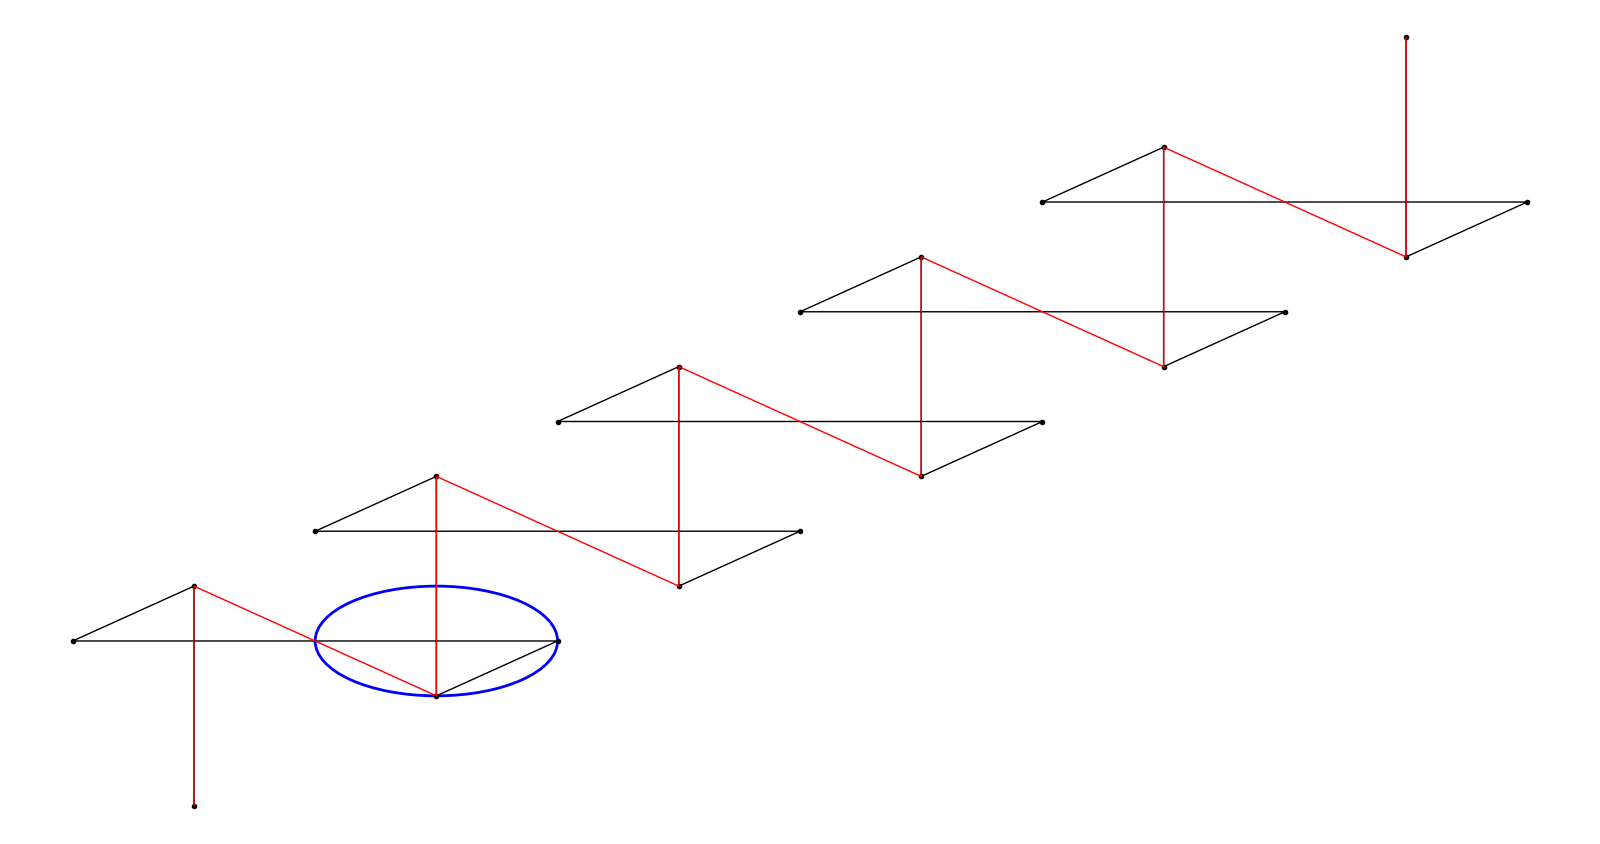
\includegraphics[scale=0.3]{./figures/local-global-bigdiff.png}
	\caption{Construction from \cref{thm:lg-approx} with \(i = 5\), a polyline consisting of multiple ``4"s. The local simplification contains all points and the global one is marked in red. The circle in blue has radius \(\varepsilon = 2\) and is centered around the self-intersection of the polyline.}
  \label{fig:local-global-bigdiff}
\end{figure}

Interestingly, in our example, if we were to define the size of a simplification to not count the start and end point then a factor of \(c_2 = 2\) would be achieved. Every simplification must contain the start and endpoint, thus, when comparing their sizes, it could make sense to ignore those points.

\subsection{A First Simplification Algorithm}
We conclude this section with a simple simplification algorithm for both the local and global Fréchet variants under any distance. This, however, only covers the case \(\varepsilon = 0\).

We know that \(\delta(u, v) = 0\) if and only if \(u = v\) for two points \(u\) and \(v\). A similar condition holds for polylines.

\begin{lemma}\label{lem:polyline_dist0}
	Let \(P\) and \(Q\) be polylines of length \(p\) and \(q\), respectively. Then \(\delta^F(P, Q) = 0\) if and only if there exists \(k \in \N\) with \(k \leq \min(p, q)\) and strictly increasing functions \(f:\set{0,\dots,k} \to \set{0,\dots,p}\) and \(g:\set{0,\dots,k} \to \set{0,\dots,q}\) with \(f(0) = g(0) = 0\), \(f(k) = p\), and \(g(k) = q\) such that:
	\begin{enumerate}
		\item \(P(f(t)) = Q(g(t))\) for all \(t \in \set{0, \dots, k}\).
		\item For each \(\ell \in \set{1, \dots, k}\) and each integer \(i\) with \(f(\ell-1) < i < f(\ell)\), there exists \(t_i \in [0,1]\) such that \(P(i) = (1-t_i)P(f(\ell-1)) + t_iP(f(\ell))\), and the sequence \(t_i\) is non-decreasing in \(i\).
		\item For each \(\ell \in \set{1, \dots, k}\) and each integer \(i\) with \(g(\ell-1) < i < g(\ell)\), there exists \(t_i \in [0,1]\) such that \(Q(i) = (1-t_i)Q(g(\ell-1)) + t_iQ(g(\ell))\), and the sequence \(t_i\) is non-decreasing in \(i\).
	\end{enumerate}
\end{lemma}

\begin{proof}
	(\(\Rightarrow\)) First, Assume \(\delta^F(P, Q) = 0\). Then there exist continuous, non-decreasing functions \(f'~:~[0,1]~\to~[0,p]\) and \(g':[0,1] \to [0,q]\) such that \(P(f'(t)) = Q(g'(t))\) for all \(t \in [0,1]\). \newline Let \(U = \set{u \mid u = P(i) = Q(j) \text{ for some } i=0,\dots,p, j=0,\dots,q}\). Define \(k = |U| - 1\), and let \(f\) and \(g\) map indices to the points in \(U\) in order. This satisfies Property (1).

	For Properties (2) and (3), the Fréchet condition ensures that between consecutive points in \(f\) (or \(g\)), the polyline must consist of a single line segment without bends, and the points on these segments must be in order. If there were multiple segments or out-of-order points, the Fréchet distance could not be zero.

	(\(\Leftarrow\)) If the conditions hold, the polylines are identical up to the addition of points on line segments. It is straightforward to construct functions \(f'\) and \(g'\) such that \(P(f'(t)) = Q(g'(t))\) for all \(t \in [0, 1]\).
\end{proof}

According to \cref{lem:polyline_dist0}, two polylines have Fréchet distance zero if and only if they differ only by points that lie on the line segments of the polyline. In other words, by removing all collinear points, the polylines become identical.

This leads to a linear-time algorithm for optimal simplification when \(\varepsilon = 0\). The start and end points must be included. For each intermediate point, we test if it lies on the line segment between its neighbors. If not, it is added to the simplification; otherwise, it is skipped.

\begin{algorithm}[ht]
  \DontPrintSemicolon
  \KwData{Polyline \(P\) of length \(n\)}
  \KwResult{Smallest \(0\)-simplification of \(P\)}
  \BlankLine
	\(simplification \gets [0]\)\;
	\For{\(i=1\) \KwTo \(n - 1\)}{
		\If{\(P(i)\) does not lie on \(\overline{P(i-1)P(i+1)}\)}{
			\(simplification.\text{append}(i)\)
		}
	}
	\(simplification.\text{append}(n)\)
	\Return{\(simplification\)}
  \caption{PolylineSimplificationWithEpsilon0(\(P\))}
  \label{algo:simplify_epsilon0}
\end{algorithm}

Testing if a point lies on a line segment is straightforward. For completeness, we derive the condition. A point \(p\) lies on \(\overline{uv}\) if and only if there exists \(t \in [0,1]\) such that \(p = u + t(v-u)\), or equivalently, \(p - u = t(v-u)\). Thus, for all coordinates \(i\), we need \(t = (p_i - u_i)/(v_i - u_i)\) to be the same. To avoid division by zero, we can reformulate this as \((p_{i-1} - u_{i-1})(v_i - u_i) = (p_i - u_i)(v_{i-1} - u_{i-1})\) for all \(i \geq 1\). To ensure \(t \in [0, 1]\), we require \(u_i \leq p_i \leq v_i\) (or \(v_i \leq p_i \leq u_i\)) for any coordinate where \(u_i \neq v_i\).
